
\chapter{Coleta de Dados} % (fold)
\label{cha:coleta_de_dados}

\section{Tempo} % (fold)
\label{sec:tempo}

A coleta de tempo de performance de um software é árdua. A estimativa de tempo depende das otimizações que o compilador pode vir a fazer para a arquitetura, memoria disponível, aplicativos rodando em concorrência, temperatura do hardware, etc. No intuito de simplificar o processo de estimativa de tempo, foi utilizado a mediana de uma serie de chamadas da aplicação. Segundo \citeonline{dolan2002benchmarking}, esta solução pode vir ser a melhor para um ponto geral de $25\%$ das possíveis alternativas de coletas de dados. Assim sendo, o \autoref{scriptods} foi uma solução desenvolvida que permitisse deixar a maquina com tempo dedicado para a aquisição de dados.

Para o funcionamento do \textit{script}, as variáveis {\code MAX} e {\code \_MAX\_THREADS} devem ser definidas com a quantidade de dados que se deseja coletar e a quantidade máxima de \textit{threads} que devem ser levantadas para a chamada do processo respectivamente. Usar uma quantidade superior a quantidade de \textit{cores}  da maquina pode produzir valores com baixa confiabilidade, visto a concorrência gerada pelas \textit{threads}. Como parâmetros, foram escolhidos $150$ dados com $7$ \textit{threads}, possibilitando haver ao menos $1$ \textit{core} livre. Para maior dinamismo da coleta dos dados, o \textit{script} é responsável por realizar a troca das \textit{branchs} onde estão localizadas as possíveis soluções e a compilação e concentração dos dados em uma planilha do \textit{LibreOffice Calc}. Assim, os algoritmos nunca são executados em concorrência, porém os dados serão coletado sob a demanda da $CPU$ em que o \textit{script} é executado.

No intuito de coletar o tempo pontual do algoritmo, o \autoref{libtime} foi desenvolvido a fim de ser usado como cronometro. O algoritmo desenvolvido com o auxilio da biblioteca {\code Chrono}\footnote{A biblioteca é disponibilizada no {\code C++11} sob o \textit{namespace} {\code std::crono::}.} permite a captura do intervalo de tempo com ate $9$ casas decimais de segundos (nanosegundos), todavia foi utilizado a precisão de microssegundos apenas, visto que o intervalo de nanosegundos não iria gerar alto impacto na diferença dos valores. Os métodos {\code begin} e {\code end} da classe são utilizados para pontuar os intervalos onde o tempo deve ser contado. O resultado da contagem pode ser obtido com o retorno do método {\code end} ou com a chamada do {\code currenttime}, dedicado apenas para o retorno deste valor.

\section{Memoria}

Para a coleta de memoria, foi utilizado o {\code valgrind} com o auxilio da ferramenta {\code massif}. Devido a haver uma criação de \textit{hash} de forma  algebrica e o método de \textit{KMP} faz uso de um autômato finito deterministico, a previa repetição das buscas com apenas $10$ ciclos já apontavam não haver a variação do gasto de memoria.
% section tempo (end)
% chapter coleta_de_dados (end)


\chapter{Analise de Resultados} % (fold)
\label{cha:analise_de_resultados}

\section{Algorítimos de \textit{string matching} exatos} % (fold)
\label{sec:algor_timos_de_string_matching_exatos}

Para a busca com algorítimos de \textit{string matching} exatos, foram considerado três métodos distintos:

\begin{description}
	\item[Expressão Regular:] Método atual de como a verificação é realizada atualmente. Foi previamente comentado na sessão de \nameref{sec:algoritimos_de_textit}.
	\item[Knuth-Morris-Pratt:] Método que faz de uso do conceito de autômatos de estados para agilizar a busca. Previamente apresentado na sessão \nameref{ssub:knuth_morris_pratt_}.
	\item[Rabin-Karpin:]  Método que faz de uso de \textit{hash}. Foi previamente comentado na sessão \nameref{ssub:rabin_karp}.
\end{description}

Após a coleta de $150$ chamadas de cada pacote usando os algoritimos apontados acima, a \autoref{ssub:rabin_karp} foi criada contendo a médiana dos tempos de execução de cada método para os pacotes selecionados.

\begin{figure}[htbp]
  \centering
  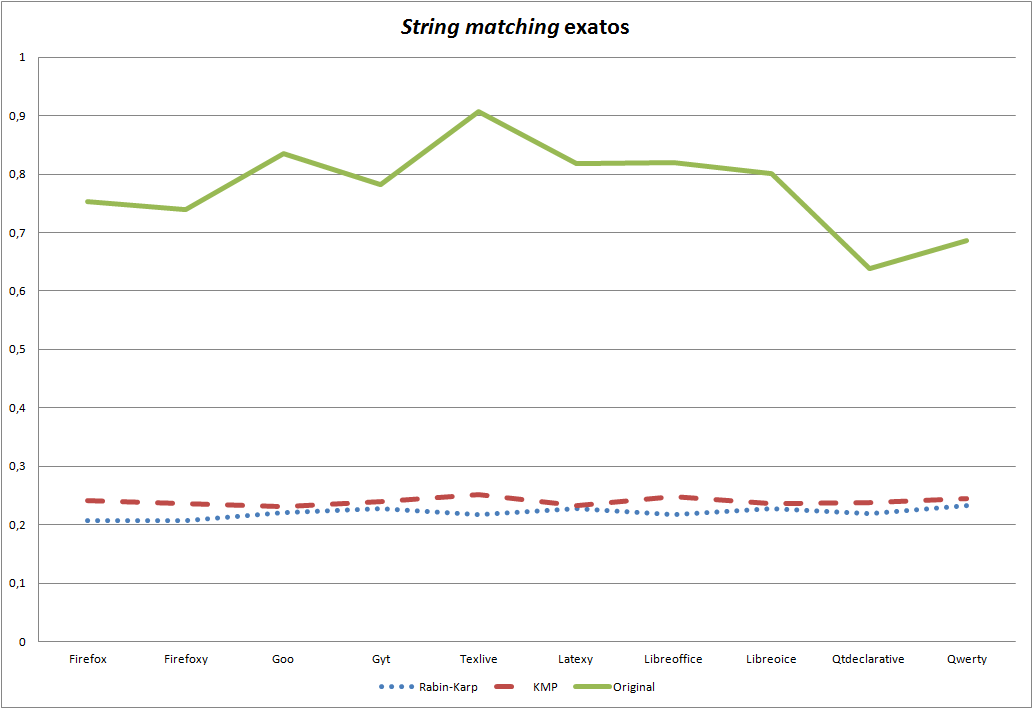
\includegraphics[width=0.95\textwidth]{figuras/tempo-rk_kmp_std}
  \caption{Estimativa de tempo para pacotes usando algorítimos de busca exata}
  \label{tempo_rk_kmp_std}
\end{figure}

Como podemos observar, tanto o \textit{Rabin-Karpin} quanto o \textit{KMP} tiveram um rendimento de cerca de $\frac{1}{3}$ do tempo gasto atualmente com o uso de expressões regulares, sendo no tempo geral, o método de \textit{Rabin-Karpin} possui um desempenho ligeiramente melhor.

% chapter analise_de_resultados (end)
